% !TeX root = RJwrapper.tex
\title{Mosaic Plots in the ggplot2 Framework ggmosaic}
\author{by Haley Jeppson, Heike Hofmann}

\maketitle

\abstract{%
The options of graphical methods for categorical variables are not well
developed in comparison to what is available for numeric variables. One
method of visualizing multidimensional data is through a mosaic plot.
Mosaic plots can be an easy and powerful option for identifying
relationships between multiple variables. However, while mosaic plots
have been implemented in a variety of packages, the ordinary grammar of
graphics does not support mosaic plots. With the R package ggmosaic, a
custom ggplot2 geom designed for mosaic plots is implemented. Equipped
with the functionality and flexibility of ggplot2, ggmosaic creates
plots that can be converted into interactive plotly graphs. This paper
provides an overview of the implementation and examples that highlight
the versatility and ease of use of ggmosaic while demonstrating the
practicality of mosaic plots.
}

\subsection{Introduction}\label{introduction}

The options of graphical methods for categorical variables are not well
developed in comparison to what is available for numeric variables.
\ldots{}elaborate\ldots{}

One method of visualizing multidimensional data is through a mosaic
plot. Mosaic plots can be an easy and powerful option for investigating
and exploring relationships between multiple variables. A mosaic plot is
constructed hierarchically with alternating spines, therefore allowing
the hierarchical structure of the counts and proportions to be
visualized. The hierarchical structure of counts and proportions is an
important concept for understanding the multivariate discrete
distribution. In a mosaic plot, the area of each graphical element is
proportional to the underlying probability of that category resulting in
a convenient graphical summary of the conditional distributions in a
contingency table. This allows us to easily visualize how the joint
distribution is composed of the product of the conditional and marginal
distributions -- which, in turn, allows us to see any association that
may be occurring between the variables. Mosaic plots excel at depicting
part-to-whole relationships. They work by combing these simple, low
dimensional graphical primitives in order to display complex,
high-dimensional data. Additionally, from a whole dataset, there tend to
be many dimensions across which to split the data into parts.

The remainder of this paper will focus heavily on mosaic plots,
beginning with an introduction to the \texttt{ggmosac} package, and
following with an overview of the implementation and examples that
highlight the versatility and ease of use of ggmosaic while
demonstrating the practicality of mosaic plots. Lastly, a review of the
multiple packages available for mosaic plots will be provided.

\subsection{ggmosaic}\label{ggmosaic}

While mosaic plots have been implemented in a variety of packages in R
\citep{R2016}, the ordinary grammar of graphics does not support mosaic
plots. However, with version 2.0.0 of \texttt{ggplot2} \citep{ggplot2},
a way for other R packages to implement custom geoms was introduced
allowing for(bringing forth?) an expansion of the utility of ggplot2. In
turn, the increasingly popular ggplot2 will likely appeal to a larger
user base. By creating a ggplot2 implementation, we hope to appeal to
this user base. Additionally, for these users, having mosaic plots
within the ggplot2 framework allows for a decrease in the amount of
syntax required in order to produce a mosaic plot.

With the R package \texttt{ggmosaic}, a custom ggplot2 geom designed for
mosaic plots is implemented. Designed to create visualizations of
categorical data, the \texttt{ggmosaic} package and has the capability
to produce bar charts, stacked bar charts, mosaic plots, and double
decker plots and therefore offers a wide range of potential plots.
Additionally, equipped with the functionality and flexibility of
ggplot2, there are many features that can be customized in
\texttt{ggmosaic}, including the type of partitioning, the ordering of
variables, conditioning on a variable, faceting, and the spacing between
the categories. The \texttt{ggmosaic} package can be installed from
\url{https://github.com/haleyjeppson/ggmosaic}.

\texttt{ggmosaic} was created primarily using \texttt{ggproto} and the
\texttt{productplots} package which was created by \citet{productplots}.
They refer to their framework as product plots, alluding to the
computation of area as a product of height and width, and the
statistical concept of generating a joint distribution from the product
of conditional and marginal distributions. To begin, \texttt{ggmosaic}
began as a geom extension of the \texttt{rect} geom with the data
handling provided in the \texttt{productplots} package which calculates
\texttt{xmin}, \texttt{xmax}, \texttt{ymin}, and \texttt{ymax} for the
\texttt{rect} geom to plot.

Having a geom designed for mosaic plots does more than simply allow us
to utilize the ggplot2 customization options such as faceting and
layering, it allows for a \texttt{ggplotly()} hook so we can create
interactive mosaic plots. Although the \texttt{ggplotly()} function
translates most of the geoms bundled with the \texttt{ggplot2} package,
it has no way of knowing about the rendering rules for custom geoms. The
\texttt{plotly} package does, however, contain the infrastructure to
provide translations of custom geoms to plotly. In \texttt{ggplot2},
many geoms are special cases of other geoms. For
example,\texttt{geom\_line()} is equivalent to \texttt{geom\_path()}
once the data is sorted by the \texttt{x} variable. \citet{carson}
Because GeomMosaic can be reduced to the lower-level geom GeomRect, we
were able to write a method for the \texttt{to\_basic()} generic
function in \texttt{plotly}.

\texttt{ggmosaic} does not come without its own set of limitations and
the main hurdle \texttt{ggmosaic} faces is that \texttt{ggplot2} is not
capable of handling a variable number of variables. The current solution
is to read in the variables \texttt{x1} and \texttt{x2} as
\texttt{x = product(x1, x2)}. The \texttt{product} function accomodates
the one or more variables by creating a list of the variables specified
which allows for it to pass \texttt{check\_aesthetics}, and then splits
the variables back into a dataframe for the calculations.

In order to fit ggmosaic within the ggplot2 framework, we must be able
to create the formula from the aestheics defined in a call. In essence,
the aesthetics set up the formula that determines the how the joint
distribution will be broken down. In geom\_mosaic, the following
aesthetics can be set:

\begin{itemize}
\item weight: select a weighting variable
\item \texttt{x}: select variables to add to formula
    \begin{itemize}
    \item declared as \texttt{x = product(x1, x2, ...)}
    \end{itemize}
\item \texttt{fill}: select a variable to be filled
    \begin{itemize}
    \item if the variable is not also called in \texttt{x}, it will be added to the formula in the first position
    \end{itemize}
\item \texttt{alpha}: select a variable to receive a transparency-scale
    \begin{itemize}
    \item if the variable is not also called in \texttt{x}, it will be added to the formula in the first position
    \end{itemize}    
\item \texttt{conds} : select a variable to condition on
\end{itemize}

These values are then sent through \texttt{productplots} functions to
create the desired formula:
\texttt{weight $\sim$ alpha $+$ fill $+$ x $|$ conds }. It should be
noted that because the plot is constructed hierarchically, the ordering
of the variables is very important.

The other parameters that can be set include the \texttt{offset} and the
\texttt{divider}. When there is a variable with many categories, it may
be of interest to decrease the size of the spacing between the spines.
This can be achieved by declaring \texttt{offset =}. The default setting
is \texttt{offset = 0.01}. There are two main ways to partition the area
- into bars or into spines. When the area is partitioned into bars, the
height is proportional to value and the width equally divides the space.
Bars can be arranged horizontally (``hbar'') or vertically (``vbar'').
Alternatively, the space can be partitioned into spines, where the width
is proportional to value, height occupies full range. Spines are space
filling and can be arranged horizontally (``hspine'') or vertically
(``vspine''). In \texttt{ggmosaic}, the type of partitioning desired can
be specified by setting \texttt{divider = " "}. The default divider for
one variable is ``hspine''. When more than one variable is to be
considered, a type of partition needs to be selected for each variable.
By selecting \texttt{divider = mosaic()}, the default, or
\texttt{divider = ddecker()}, the correct number of partitions will be
selected. For example, if three variables were to be plotted, the
default, \texttt{divider = mosaic()}, would partition the plot with
spines in alternating directions, beginning with a horizontal spine,
i.e. \texttt{divider = c("hspine", "vspine", "hspine")}. It is also an
option to manually select the type of partition that will be used for
each variable, i.e. \texttt{divider = c("hbar", "vspine", "hspine")}. It
should be noted that the first partition in the vector will be the last
partition made in the plot. As mentioned above, when no divider is
declared, the default \texttt{divider = mosaic()} will begin with a
horizontal spine and alternate directions with each subsequent variable.

To demonstrate some of the capabilities of \texttt{ggmosaic}\ldots{}

\subsection{Examples}\label{examples}

We will examine a couple of data sets while emphasizing the versatility
and ease of use of \texttt{ggmosaic}. The topic selected to \ldots{} has
been a hot topic in the new recently - Airline dissatisfaction. First,

\subsubsection{Shrinking Seats}\label{shrinking-seats}

\begin{Schunk}


\begin{center}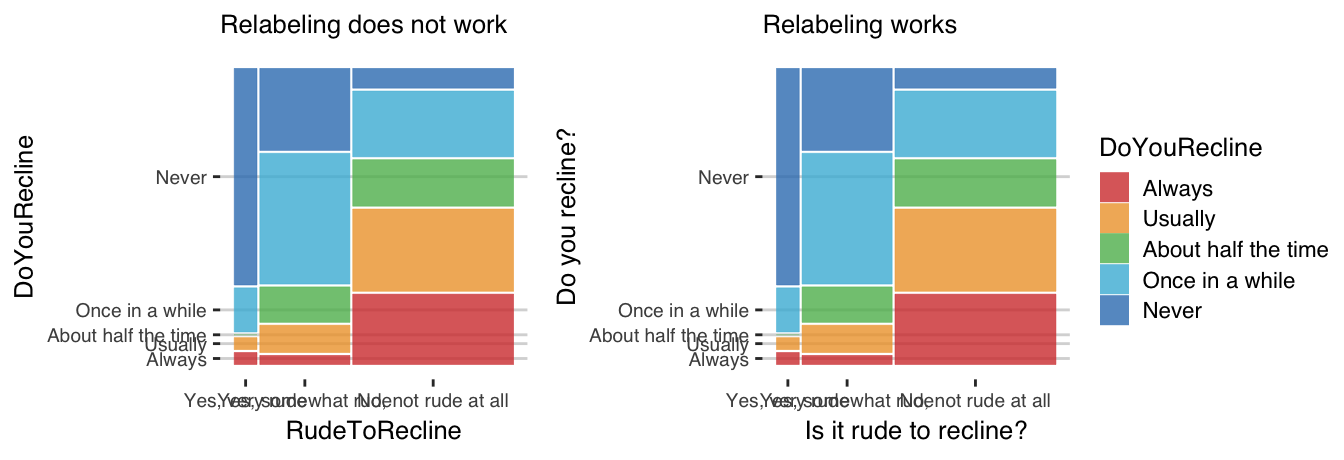
\includegraphics[width=0.5\linewidth]{fly_files/figure-latex/unnamed-chunk-1-1} \end{center}

\end{Schunk}

\begin{Schunk}


\begin{center}\includegraphics[width=0.5\linewidth]{fly_files/figure-latex/unnamed-chunk-2-1} \end{center}

\end{Schunk}

\begin{Schunk}


\begin{center}\includegraphics[width=0.5\linewidth]{fly_files/figure-latex/unnamed-chunk-3-1} \end{center}

\end{Schunk}

\subsubsection{Airline Ettiquette}\label{airline-ettiquette}

Is there a social contract we should all be following when flying? Who
gets to use that extra arm rest? Is it okay to recline your seat or to
bring your baby or child on board? Are people upset if the child is
unruly and, like Donald Trump, wish to ``get that baby out of here?''
\citep{cnn} How often are you allowed to leave your seat before being
perceived as rude? Does the occupant of the window seat reserve all
rights to the window shade? And is it okay to switch seats for family,
friends, or to an unsold seat?

To learn a little about people's opinions on what is considered to be
rude behavior while on an airplane, FiveThirtyEight ran a SurveyMonkey
Audience poll for two days in August of 2014. \citep{fivethirtyeight}
The survey had 1,040 respondents (874 of whom had flown) aged 18-60+
from across the county and asked twenty-six questions that ranged from
background information regarding the respondent to feelings regarding
potentially aggravating behavior one might encounter on an airplane. The
data set is available from FiveThirtyEight's data git hub repository.

To explore the data a bit more, I used the \texttt{ggmosaic} package.
The original analysis done by FiveThirtyEight focused primarily on the
perceived rudeness of a behavior, one behavior at a time, or comparing
the response ``Very Rude'' across all behaviors. By using a mosaic plot,
multiple categorical counts can be viewed simultaneously which will
provide a clearer view of the underlying data and allow for more
comparisons to be made. We can perhaps gain more insight into how the
seat recliner, the chatterbox, or the unruly child is perceived and how
those perceptions may be related.

I began by taking a look at who is flying and how frequently they fly.
In addition to answering questions about common aggravating behaviors,
the respondents answered questions regarding their demographics. Some of
the demographic types of questions asked included age, gender, household
income bracket, education level and region.

Figure \textasciitilde{}\ref{fig: who1} was created by first dividing
the space into horizontal spines each representing the proportion of
respondents within that household income bracket. We can view these
horizontal spines in the final product and they will answer questions
such as, ``what proportion of the respondents have a household income of
under \$100,000?'' The next step was to split each horizontal spine into
vertical spines, which were subsequently filled with different colors,
representing how frequently one flew. This plot can be used to answer
questions such as ``what proportion of those that have a household
income of under \$24,999 flies a few times per month?''

\begin{Schunk}


\begin{center}\includegraphics[width=0.5\linewidth]{fly_files/figure-latex/unnamed-chunk-4-1} \end{center}

\end{Schunk}

From Figure \textasciitilde{}\ref{fig: who1} we can see that the largest
majority of the survey participants fall within the household income
bracket of \$50,000-99,000, and that as household income increases, the
more likely one is to frequently fly. Even more interesting, the few
participants that responded that they flew every day were of the two
lower income brackets or chose to not respond to the question.

\begin{Schunk}


\begin{center}\includegraphics[width=0.5\linewidth]{fly_files/figure-latex/who2-1} \end{center}

\end{Schunk}

Continuing the investigation into who is flying and how frequently they
fly, Figure \textasciitilde{}\ref{fig: who2} presents how frequently the
respondents flew by education level. From the mosaic plot, we can see
that the majority of respondents had some type of college education and
there is a trend people flying more frequently as education level
increases.

\begin{Schunk}


\begin{center}\includegraphics[width=0.5\linewidth]{fly_files/figure-latex/who3-1} \end{center}

\end{Schunk}

To add to this, Figure \textasciitilde{}\ref{fig: who3} shows that
gender and age don't play too large of a role in how often one flies,
though interestingly the largest group of those that never fly was made
up of males in the age bracket 18-29. Figure
\textasciitilde{}\ref{fig: who3} exemplifies how having mosaic plots
implemented as a geom allows for the ggplot2 customization features to
easily be accessed. Here, rather than partitioning into spines for the
gender categories, I have faceted on gender. Statistically, this relates
to conditioning on the variable on gender. The distribution that is
being displayed by Figure \textasciitilde{}\ref{fig: who3} is
f(FlightFreq, Age \textbar{}Gender)

\begin{Schunk}


\begin{center}\includegraphics[width=0.5\linewidth]{fly_files/figure-latex/recline1-1} \end{center}

\end{Schunk}

Next I dove into the perceived level of rudeness of some of the more
common behaviors. First up, how do the participants view ``The seat
recliner'' and are the participants seat recliners themselves? As
airlines look to shrink costs, the airline seats appear to be shrinking
as well. In the past thirty years, the average cheap seat has shrank
from 18 inches wide to about 16 and a half inches wide. \citet{washpost}
Has this smaller space brought strong opinions on a flight passenger's
right to recline their seat? We can look at how often the participants
reclined their seat and also at how rude participants believe the
behavior to be. However, perhaps a more interesting question is ``How
often does one recline given they feel the behavior is very rude?''
Figure \textasciitilde{}\ref{fig: recline} is a breakdown of participant
responses to the two questions ``Do you recline?'' and ``Is it rude to
recline?'' that can allow for such types of questions to be answered.
While some of the results were as expected - the more rude someone
considers the act reclining, the less likely they were to recline their
own chair- there were three respondents who felt it was very rude to
recline your seat on an airplane, yet always reclined their own seat.
The plot also lets us know that the majority of the respondents do not
find it at all rude to recline your seat and are fairly evenly divided
on how often they themselves recline their own seat.

\begin{Schunk}


\begin{center}\includegraphics[width=0.5\linewidth]{fly_files/figure-latex/recline-1} \end{center}

\end{Schunk}

\begin{Schunk}


\begin{center}\includegraphics[width=0.5\linewidth]{fly_files/figure-latex/eliminate-1} \end{center}

\end{Schunk}

Not a particularly surprising revelation, but Figure
\textasciitilde{}\ref{fig: eliminate} displays how the small propotion
of participants that view the act of reclining your seat on an airplane
as rude would also like to eliminate the option of reclining. In
contrast the larger proportion that do not view the act as rude do not
see a reason to eliminate the option.

Next, how did the participants view babies and unruly children on
flights? Are there certain demographics that are more likely to be
offended by their presence? Are parents less likely or more likely to be
offended by other children? The firstplot adressing this topic is Figure
\textasciitilde{}\ref{fig: baby}. Here we can get an idea of how the
particpiants viewed the act of bringing a baby on an aircraft.
Fortunately, we see that most were not bothered, but there is a slight
proportion that finds it to be very rude.

To see where those respondents might be coming from, the next plot looks
at how the participants judged the level of rudeness of bringing a baby
on board broken down by whether the participant had a child under the
age of 18 and then by gender. \ref{fig: baby2} is an example of one of
the other types of plots \texttt{ggmosaic} is capable of creating, a
double decker plot. A modification of a mosaic plot, a double decker
plot, is composed of n-1 hspines and ends with a vspine rather than
alternating hspines and vspines. In \textasciitilde{}\ref{fig: baby2},
the plot is first split horizontally by response to ``Do you have a
child under the age of 18?''. From there each hspine is split into
gender resulting in a plot where each combination of gender and child
under the age of 18 is represented by a vertical bar where the width
represents the proportion of that category. Lastly, each vertical bar is
split vertically by the responses to ``Is it rude to bring a baby on a
plane?'' The finished product is a plot that allows for the three
variables to be presented concisely and displays how the proportions
differ.

\begin{Schunk}


\begin{center}\includegraphics[width=0.5\linewidth]{fly_files/figure-latex/baby-1} \end{center}

\end{Schunk}

In \textasciitilde{}\ref{fig: baby}, we see that those without a child
under the age of 18 make up the largest proportion of the respondents
and they are more likely to consider bringing a baby on board as rude.
Additionally, men or more likely than women to consider it rude to bring
a baby on a flight.

\begin{Schunk}


\begin{center}\includegraphics[width=0.5\linewidth]{fly_files/figure-latex/baby2-1} \end{center}

\end{Schunk}

The next figure, Figure \textasciitilde{}\ref{fig: child}, looks into
how the participants viewed sharing the plane ride with an unruly child.
In Figure \textasciitilde{}\ref{fig: child} we can see that the
participants were likely to be bothered by an unruly child. Perhaps this
has to do with the wording of the question in the SurveyMonkey, but I
continued on with the analyis anyway.

\begin{Schunk}


\begin{center}\includegraphics[width=0.5\linewidth]{fly_files/figure-latex/child-1} \end{center}

\end{Schunk}

To see where those opinions stemmed from, or to see if those opinions
varied by gender and whether or not the participant has a child under
the age of 18, Figure \textasciitilde{}\ref{fig: child2} was created. In
the double decker plot, it is clear that females are more forgiving of
unruly children than males and that parents of children under the age of
18 are also more forgiving. It does, however, seem fairly clear that
most find the presence of an unruly child as rude.

\begin{Schunk}


\begin{center}\includegraphics[width=0.5\linewidth]{fly_files/figure-latex/child2-1} \end{center}

\end{Schunk}

\begin{Schunk}


\begin{center}\includegraphics[width=0.5\linewidth]{fly_files/figure-latex/age_baby-1} \end{center}

\end{Schunk}

\begin{Schunk}


\begin{center}\includegraphics[width=0.5\linewidth]{fly_files/figure-latex/age_child-1} \end{center}

\end{Schunk}

To continue the investigation of how often faircraft passengers find an
unruly child or baby on board as rude and how this opinion varies person
to person, Figures \textasciitilde{}\ref{fig: age_baby} and
\textasciitilde{}\ref{fig: age_child} were created. An interesting
revelation brought about by these two plots is that while those older
seem to be less likely to be bothered by a baby being on a flight, they
are more likely to be upset by an unruly child.

After exploring the data a bit more, it is clear that there does not
seem to be a general consensus on what passengers perceive to be
acceptable behavior on an airplane. The use of mosaic plots aided in the
exploration of how certain opinions or behaviors are related.

\subsection{Comparisons}\label{comparisons}

\begin{Schunk}


\begin{center}\includegraphics[width=0.5\linewidth]{fly_files/figure-latex/comparisons-1} \end{center}



\begin{center}\includegraphics[width=0.5\linewidth]{fly_files/figure-latex/comparisons-2} \end{center}



\begin{center}\includegraphics[width=0.5\linewidth]{fly_files/figure-latex/comparisons-3} \end{center}

\end{Schunk}

\subsection{Conclusion}\label{conclusion}

\subsection{Summary}\label{summary}

This file is only a basic article template. For full details of
\emph{The R Journal} style and information on how to prepare your
article for submission, see the
\href{https://journal.r-project.org/share/author-guide.pdf}{Instructions
for Authors}.

\bibliography{RJreferences}

\address{%
Haley Jeppson\\
Iowa State University\\
line 1\\ line 2\\
}
\href{mailto:author1@work}{\nolinkurl{author1@work}}

\address{%
Heike Hofmann\\
Iowa State University\\
line 1\\ line 2\\
}
\href{mailto:author2@work}{\nolinkurl{author2@work}}

